% \documentclass[a4paper, 11pt]{article}
\documentclass{article}

\usepackage[dvipsnames]{xcolor}
\usepackage{ctex}
\usepackage{graphicx}
\usepackage[unicode]{hyperref}
\usepackage{cite}
\usepackage{indentfirst}
\usepackage{listings}
\usepackage{geometry}
\usepackage{amsmath}
\usepackage{tabularx}

\geometry{a4paper, left=2cm, right=2cm, top=1cm, bottom=1.5cm}

% \lstset{
%   language=C++,
%   basicstyle=\fontsize{8}{5}\ttfamily, % 设置代码字体大小为 12pt
%   breaklines=true, % 自动换行
%   numbers=left,
%   showstringspaces = false
% }

%%%%%% 设置字号 %%%%%% 
\newcommand{\chuhao}{\fontsize{nn42pt}{\baselineskip}\selectfont}
\newcommand{\xiaochuhao}{\fontsize{36pt}{\baselineskip}\selectfont}
\newcommand{\yihao}{\fontsize{28pt}{\baselineskip}\selectfont}
\newcommand{\erhao}{\fontsize{21pt}{\baselineskip}\selectfont}
\newcommand{\xiaoerhao}{\fontsize{18pt}{\baselineskip}\selectfont}
\newcommand{\sanhao}{\fontsize{15.75pt}{\baselineskip}\selectfont}
\newcommand{\sihao}{\fontsize{14pt}{\baselineskip}\selectfont}
\newcommand{\xiaosihao}{\fontsize{12pt}{\baselineskip}\selectfont}
\newcommand{\wuhao}{\fontsize{10.5pt}{\baselineskip}\selectfont}
\newcommand{\xiaowuhao}{\fontsize{9pt}{\baselineskip}\selectfont}
\newcommand{\liuhao}{\fontsize{7.875pt}{\baselineskip}\selectfont}
\newcommand{\qihao}{\fontsize{5.25pt}{\baselineskip}\selectfont}

% %%%% 设置 section 属性 %%%%
% \makeatletter
% \renewcommand\section{\@startsection{section}{1}{\z@}%
% {-1.5ex \@plus -.5ex \@minus -.2ex}%
% {.5ex \@plus .1ex}%
% {\normalfont\sihao\CJKfamily{hei}}}
% \makeatother

 %%%% 设置 subsection 属性 %%%%
% \makeatletter
% \renewcommand\subsection{\@startsection{subsection}{1}{\z@}%
% % {-1.25ex \@plus -.5ex \@minus -.2ex}%
% % {-1ex \@plus -.5ex \@minus -.2ex}%
% {-1ex \@plus -.3ex \@minus -.1ex}%
% {.4ex \@plus .1ex}%
% {\normalfont\xiaosihao\CJKfamily{hei}}}
% \makeatother

% %%%% 设置 subsubsection 属性 %%%%
% \makeatletter
% \renewcommand\subsubsection{\@startsection{subsubsection}{1}{\z@}%
% {-1ex \@plus -.5ex \@minus -.2ex}%
% {.3ex \@plus .1ex}%
% {\normalfont\xiaosihao\CJKfamily{hei}}}
% \makeatother

%%%% 段落首行缩进两个字 %%%%
\makeatletter
\let\@afterindentfalse\@afterindenttrue
\@afterindenttrue
\makeatother
% \setlength{\parindent}{2em}  %中文缩进两个汉字位

%%%% 下面的命令重定义页面边距,使其符合中文刊物习惯 %%%%
% \addtolength{\topmargin}{-54pt}
% \setlength{\oddsidemargin}{0.63cm}  % 3.17cm - 1 inch
% \setlength{\evensidemargin}{\oddsidemargin}
% \setlength{\textwidth}{14.66cm}
% \setlength{\textheight}{24.00cm}    % 24.62

%%%% 下面的命令设置行间距与段落间距 %%%%
\linespread{1.0}
% \setlength{\parskip}{1ex}
\setlength{\parskip}{0.5\baselineskip}

% 在导言区进行样式设置
\lstset{
    language=C++, % 设置语言
 	basicstyle=\ttfamily, % 设置字体族
 	breaklines=true, % 自动换行
 	keywordstyle=\bfseries\color{NavyBlue}, % 设置关键字为粗体,颜色为 NavyBlue
 	morekeywords={PressureSensor, Button, Oled}, % 设置更多的关键字,用逗号分隔
 	emph={self}, % 指定强调词,如果有多个,用逗号隔开
    emphstyle=\bfseries\color{Rhodamine}, % 强调词样式设置
    commentstyle=\itshape\color{black!50!white}, % 设置注释样式,斜体,浅灰色
    stringstyle=\bfseries\color{PineGreen!90!black}, % 设置字符串样式
    columns=flexible,
    numbers=left, % 显示行号在左边
    numbersep=2em, % 设置行号的具体位置
    numberstyle=\footnotesize, % 缩小行号
    % frame=single, % 边框
	tabsize = 4,  %行缩进
    framesep=1em % 设置代码与边框的距离
}

%%%% 正文开始 %%%%
\begin{document}	
		%%%% 定理类环境的定义 %%%%
\newtheorem{example}{例}             % 整体编号
\newtheorem{algorithm}{算法}
\newtheorem{theorem}{定理}[section]  % 按 section 编号
\newtheorem{definition}{定义}
\newtheorem{axiom}{公理}
\newtheorem{property}{性质}
\newtheorem{proposition}{命题}
\newtheorem{lemma}{引理}
\newtheorem{corollary}{推论}
\newtheorem{remark}{注解}
\newtheorem{condition}{条件}
\newtheorem{conclusion}{结论}
\newtheorem{assumption}{假设}

		%%%% 重定义 %%%%
\renewcommand{\contentsname}{目录}  % 将Contents改为目录
\renewcommand{\abstractname}{摘要}  % 将Abstract改为摘要
\renewcommand{\refname}{参考文献}   % 将References改为参考文献
\renewcommand{\indexname}{索引}
\renewcommand{\figurename}{图}
\renewcommand{\tablename}{表}
\renewcommand{\appendixname}{附录}
\renewcommand{\algorithm}{算法}	

		%%% 定义标题格式,包括title,author,affiliation,email等 %%%%
\title{智能仓储系统的开发研究}
% \author{XXX\footnote{电子邮件: XXXXXXXXXXXX@zjut.edu.cn 学号: XXXXXXXXXXXX}\\[2ex]
% \xiaosihao 浙江工业大学\\[2ex]}
\author{\xiaosihao 先进计算与机器人研究所}
%\date{}
		
		%%%% 以下部分是正文 %%%%  
\maketitle
		
\tableofcontents
\newpage

\section{第一章: 压力测量模块}
\begin{figure}[h]
	\centering
	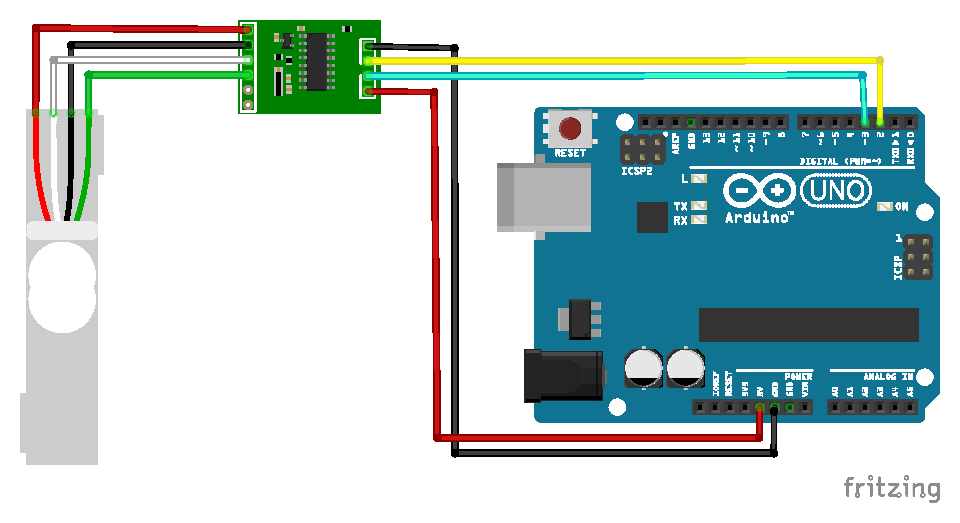
\includegraphics[width=\linewidth]{../Picture/PressureSensor.pdf}
	\caption{压力测量模块流程}
	\label{fig:压力测量模块流程图}
	\hfill
\end{figure}
		
	压力测量模块的连线:
\begin{itemize}
	\item 称重传感器的红线代表电源正极, 连接HX711 模块的 E+ 引脚
	\item 称重传感器的黑线代表电源负极, 连接HX711 模块的 E- \hspace{0.5em}引脚
	\item 称重传感器的白线代表信号输出, 连接HX711 模块的 A- \hspace{0.5em}引脚
	\item 称重传感器的绿线位保留线, 连接HX711 模块的 A+ 引脚		
	\item HX711 模块的GND引脚连接 arduino 的GND引脚
	\item HX711 模块的VCC引脚连接 arduino 的5V引脚
	\item HX711 模块的DT\hspace{0.5em} 引脚连接arduino的任意数字引脚pin\_DT(下文为数字引脚3), 在构造函数里会将Arduino中的该引脚
	设置为输入模式, 用于接收HX711传来的数字信号。
	\item HX711 模块的SCK引脚连接 arduino 的任意数字引脚pin\_SCK(下文为数字引脚2), 在构造函数里会将Arduino中的该引脚设置为输出模式,
	用于发送脉冲, 然后HX711会按数位输出数据到pin\_DT。
\end{itemize}

初始秤的计算步骤
\begin{itemize}
  \item 1. 获得空秤时的AD值, 并除以Gapvalue;
  \item 2. 获得放了物体后的AD值, 并除以Gapvalue;
  \item 2. 相减后即得到理论质量;
\end{itemize}

在上述计算步骤中, 最常用到的就是读取AD值这个函数, 而且在得到空秤后的AD值, 需要储存便于之后相减的运算。所以我们需要一个类来封装上述读取的方法
和读取后的变量。 \par
\begin{itemize}
  \item 在基类HX711中只有读取AD值的方法, 也就是第一二步中的前半部分;
  \item 在基于HX711的派生类Surface中还有计算Gapvalue和储存AD值相关的方法, 也就是第一二步中的后半部分;
  \item 在基于Surface的派生类PressureSensor中有计算步骤中第三步的方法。
\end{itemize} 
这样三个类刚好实现了这三步初始秤的计算, 并且每一个类的使用都有简洁的ino文件来演示。 \par
在这三个类中的方法取名主要是"Get", "Set", "Output"这三种, "Get"是用来计算返回一个值, "Set"是用来将Get返回的值保存到类中的某一个变量中, 
"Output"是用来将某一变量的值打印在串口。

\subsection{HX711}
HX711类的核心变量是HX711value, 因为后续继承不必继承这个变量, 所以设为私有成员。
\begin{lstlisting}
#include <Arduino.h>

class HX711{
private:
  unsigned long HX711value;

public:
  int pin_SCK, pin_DT;   

  HX711(){};
  HX711(int p1, int p2);
  unsigned long Get_HX711value();
  void Set_HX711value();
  void Output_HX711();
};
\end{lstlisting}

从这一章开头的硬件连接图可以看出来, 压力测量模块除了5v和接地要连线, 要设置SCK和DT连接的数字引脚。
设置SCK和DT的数字引脚是放在HX711构造函数HX711(int p1, int p2)里,
\begin{lstlisting}
HX711::HX711(int p1, int p2){
  pin_SCK = p1;
  pin_DT = p2;
  pinMode(pin_DT, INPUT);	
  pinMode(pin_SCK, OUTPUT);	
};  
\end{lstlisting}

HX711类的中Get\_HX711value是用开发商的方法返回AD值, 具体原理放在了附录前两节。
\begin{lstlisting}
unsigned long HX711::Get_HX711value() {
  unsigned long AD_value=0;
	digitalWrite(pin_DT, HIGH);
	delayMicroseconds(1);
	digitalWrite(pin_SCK, LOW);
	delayMicroseconds(1);
  while(digitalRead(pin_DT));
   
  for(unsigned char i=0;i<24;++i) {
	  digitalWrite(pin_SCK, HIGH); 
		delayMicroseconds(1);
	  AD_value <<= 1; 
		digitalWrite(pin_SCK, LOW); 
		delayMicroseconds(1);
	  if(digitalRead(pin_DT)) ++AD_value; 
    // Serial.println(AD_value);
	} 
	// AD_value ^= 0x800000;

 	digitalWrite(pin_SCK, HIGH); 
	delayMicroseconds(1);
	digitalWrite(pin_SCK, LOW); 
	delayMicroseconds(1);

  // Serial.println(AD_value);
  return AD_value;
};  
\end{lstlisting}

Set\_HX711value是通过Get\_HX711value来更新HX711value。
\begin{lstlisting}
void HX711::Set_HX711value() {
  HX711value = Get_HX711value();
}  
\end{lstlisting}

Output\_HX711是将HX711value打印在串口。
\begin{lstlisting}
void HX711::Output_HX711() {
  Serial.print("HX711value:");
  Serial.println(HX711value);
}  
\end{lstlisting}

\subsubsection{HX711.ino}
演示代码是实现将HX711value打印在串口。
\begin{lstlisting}
#include "HX711.h"

HX711 hx711(4, 5);

void setup() {
  Serial.begin(9600);
}

void loop() {
  hx711.Set_HX711value();
  hx711.Output_HX711();
  delay(500);
}
  
\end{lstlisting}

\subsection{Surface}
Surface类的核心变量是Gapvalue和Surfacevalue, 因为后续要继承这个变量, 所以设为公共成员。
\begin{lstlisting}
#include "HX711.h"
#include <EEPROM.h>

class Surface : public HX711 {
union coeffience {
  unsigned long offboard;
  byte onboard[4];
};

public:
  unsigned long Surfacevalue;
  float Gapvalue;
  int range;

  Surface(){};
  Surface(int p1, int p2, int r);
  unsigned long Get_Surfacevalue();
  float Get_Gapvalue();
  void Set_Surfacevalue();
  void Set_Gapvalue();
  void Output_Surfacevalue();
  void Output_Gapvalue();
};
\end{lstlisting}

Surface继承HX711后, 构造函数和私有成员不能继承, 所以在Surface中重新写了构造函数Surface(int p1, int p2)。与HX711的构造函数不同的是,
这里实现了在arduino已储存了Surfacevalue时, 会直接读取。\par
\begin{lstlisting}
Surface::Surface(int p1, int p2, int r) : HX711(p1, p2){
  coeffience memory;
  for (int i=0; i<4; ++i)
    memory.onboard[i]=EEPROM.read(i);
  if (memory.offboard!=0)
    Surfacevalue = memory.offboard;

  range = r;
};
\end{lstlisting}

这个实现中有一个细节就是创建了一个共用体coeffience, 当某一共用体coeffience变量保存了任意格式的数据, 可以是unsigned long格式, 也可以是
byte*格式, 可以通过访问不同成员offboard和onboard来切换。\par
因为arduino板上由于位数限制不能直接储存unsigned long格式的数据, 需要4个地址来储存, 只能按位分成byte[4]进行储存, 所以这个共用体对arduino的数据储存十分重要。\par
关于存储Surfacevalue, 一种是存储Surface的AD值, 一种是存储除以Gapvalue后的Surfacevalue。因为AD值会一直跳动, 即使不放物体, 波动也一直存在。
所以存储AD值没有什么意义, 一有不同就会需要覆盖重写。除以Gapvalue后的值比之前小很多, 波动不会特别明显, 偶尔也需要覆盖重写, 但次数少多了, 
节约了arduino的重写次数(arduino重写次数有限)。

\begin{lstlisting}
float Surface::Get_Gapvalue(int range) {
  return 128 * 16.777215 / range;
};
\end{lstlisting}
Gapvalue的计算公式详见附录前两节, range表示传感器的量程, 当前用的是20。

Set\_Gapvalue是通过Get\_Gapvalue来更新Gapvalue。
\begin{lstlisting}
void Surface::Set_Gapvalue() {
  Gapvalue = Get_Gapvalue();
};
\end{lstlisting}

Surface类的中Get\_Surfacevalue是计算十次Surface的AD值的平均值, 除以Gapvalue后返回计算结果。
\begin{lstlisting}
unsigned long Surface::Get_Surfacevalue() {
  unsigned long AD_Sum=0, AD_Read=0;
  for (int i=0; i<10; ++i){
    AD_Read = Get_HX711value();
    AD_Sum+=AD_Read;
  }
  unsigned long value = AD_Sum/(10*Gapvalue);

  return value;
};
\end{lstlisting}

Set\_Surfacevalue是通过Get\_Surfacevalue来更新Surfacevalue, 并判断是否与arduino已储存的相同, 相同就不再覆盖写入了, 反之覆盖重写不同的地方。
\begin{lstlisting}
void Surface::Set_Surfacevalue() {
  Surfacevalue = Get_Surfacevalue();
  coeffience buffer_Surface;
  buffer_Surface.offboard = Surfacevalue;

  for(int i=1; i<4; i++)    //判断是否与上次储存的AD_Surface相同
    if (!(EEPROM.read(i)==buffer_Surface.onboard[i])) {
      Serial.println("OVERWRITE");
      EEPROM.write(i, buffer_Surface.onboard[i]);
    }  
};
\end{lstlisting}

Output\_Surfacevalue是将Surfacevalue打印在串口。
\begin{lstlisting}
void Surface::Output_Surfacevalue() {
  Serial.print("Surfacevalue:");
  Serial.println(Surfacevalue);
}
\end{lstlisting}

\subsubsection{Surface.ino}
演示代码先将Gapvalue打印在串口, 然后将Surfacevalue打印在串口。
\begin{lstlisting}
#include "Surface.h"

Surface s(4,5,20);

void setup() {
  Serial.begin(9600);
  s.Set_Gapvalue();
  s.Output_Gapvalue();
}

void loop() {
  s.Set_Surfacevalue();
  s.Output_Surfacevalue();
  delay(500);
}
\end{lstlisting}

\subsection{PressureSensor}
PressureSensor类的核心变量是Weight, 因为后续要继承这个变量, 所以设为公共成员。
\begin{lstlisting}
#include "Surface.h"

class PressureSensor : public Surface {
public:
  unsigned long Weight;

  PressureSensor(){};
  PressureSensor(int p1, int p2, int r);
  unsigned long Get_Weight();
  void Set_Weight();
  void Output_Weight();
}; 
\end{lstlisting}

PressureSensor继承Surface后, 构造函数和私有成员不能继承, 所以在PressureSensor中重新写了构造函数PressureSensor(int p1, int p2)。
除了设置SCK和DT连接的数字引脚, 还要更新好Gapvalue和Surfacevalue。\par
\begin{lstlisting}
PressureSensor::PressureSensor(int p1, int p2, int r) : Surface(p1, p2, r){
  Set_Gapvalue();
  Set_Surfacevalue();	
}
\end{lstlisting}

PressureSensor类的中Get\_Weight是先调用Get\_HX711value(), 除以Gapvalue后, 与在构造函数PressureSensor(int p1, int p2)里更新了的
Surfacevalue相减, 返回计算结果。通过if来避免这两种情形: 在没放东西的时候, 有可能AD值比一开始测得还小, 这时候就会因为出现负数的原因, 
显示一个加一取反后的很大的数; 也有可能AD值比一开始测得大一点, 显示为1, 2等较小的数。
\begin{lstlisting}
unsigned long PressureSensor::Get_Weight() {
  unsigned long difference = Get_HX711value()/Gapvalue - Surfacevalue;
  if (difference > 20000 || difference < 4) difference = 0;			
  return difference;
};
\end{lstlisting}

Set\_Weight是通过Get\_Weight来更新Weight。
\begin{lstlisting}
void PressureSensor::Set_Weight() {
  Weight = Get_Weight();
};
\end{lstlisting}

Output\_Weight是将Weight打印在串口。
\begin{lstlisting}
void PressureSensor::Output_Weight() {
  Serial.print("Weight:");
  Serial.println(Weight);
};
\end{lstlisting}

\subsubsection{PressureSensor.ino}
演示代码将Weight打印在串口。
\begin{lstlisting}
#include "PressureSensor.h"

PressureSensor ps(4,5,20);

void setup() {
  Serial.begin(9600);
  ps.Set_Surfacevalue();
}

void loop() {
  ps.Set_Weight();
  ps.Output_Weight();
  delay(500);
}
\end{lstlisting}

\subsection{上位机采集称重结果}
\subsubsection{上位机}
在上一节得到的结果中, 我们还需要验证一下和真实重量的差别有多大。为了方便保存已放置的砝码的质量数值, 用到了上位机。\par
\begin{itemize}
  \item 用户在上位机输入放入砝码的总次数, 即数组长度;
  \item 用户在上位机输入当前放在秤上的真实质量数值;
  \item 按下回车后, 等待arduino接收到信号后返回称重结果给上位机;
  \item 上位机在接收到后, 将之前输入的真实质量数值和对应称重结果分别保存到两个数组中, 然后画图显示。
\end{itemize}

\lstinputlisting{./code/uppermachine.txt}

得到的数组realweights和weights分别作为横纵坐标画散点图。理想情况下, 画出的散点图用直线$y=kx+b$拟合就能基本覆盖。
所以后续用最小二乘法来进行校准秤。为了方便日常使用的校准, 这里是在上位机中显示散点图和最小二乘法得到的直线图。

\subsubsection{DataCollect}
DataCollect类的核心作用就是接收到上位机发来的信号后称重, 并将结果返回给上位机。因为要称重, 所以肯定要用到PressureSensor类, 
后续没有这个这个类相关的继承, 所以直接将ps设为私有成员。
\begin{lstlisting}
#include "PressureSensor.h"

class DataCollect{
private:
  PressureSensor ps;

public:
  DataCollect() {};
  DataCollect(int p1, int p2, int r);
  void Output_data();
}; 
\end{lstlisting}

在构造函数DataCollect(int p1, int p2)里, 对ps进行初始化, 并更新ps中Surfacevalue。
\begin{lstlisting}
DataCollect::DataCollect(int p1, int p2, int r) {
  ps = PressureSensor(p1, p2, r);
  ps.Set_Surfacevalue();
};  
\end{lstlisting}

由于串口通信是一个字节一个字节传输, 所以当检测到串口有消息传来时, 需要先把消息用Serial.read()读完, 再进行称重, 打印结果。否则, 上位机发送
"一个"数值(其实是个字符串), 会收到多个返回值。
\begin{lstlisting}
void DataCollect::Output_data() {
  if (Serial.available()>0) {
    while (Serial.available()>0)
      Serial.read();
    ps.Set_Weight();
    ps.Output_Weight();
  }
}
\end{lstlisting}

\subsubsection{DataCollect.ino}
演示代码实现等待接收上位机信号, 称重一次, 并返回一次结果。
\begin{lstlisting}
#include "DataCollect.h"

DataCollect dc(4, 5, 20);

void setup() {
  Serial.begin(9600);
}

void loop() {
  dc.Output_data();
  delay(500);
}
\end{lstlisting}

\subsection{附录}
\subsubsection{常用函数HX711\_Read(part 1)}
HX711\_Read()是用来得到HX711AD模块读到的电压信号。HX711AD模块在连接压力传感器后, 可以将压力传感器所传出的电压信号(一种模拟信号)
转换成AD值(一种数字信号)。其内部实现是通过建立一个电压值(模拟信号)与24位的二进制数(数字信号)的对应关系表。 
在前面我们指定了与HX711\_SCK和HX711\_DT相连的引脚pin\_SCK和pin\_DT, 在HX711\_Read()中, pin\_SCK主要是输出脉冲到
HX711\_SCK, pin\_DT主要是输入HX711\_DT传来的数字信号。其中前24次脉冲分别使得pin\_DT读到二进制数的所有数位上的数。在此之后,
可以选择再进行第25次或第26次或第27次脉冲, 其作用用于确认压力传感器输入到HX711AD模块的输入通道种类(分为AB两种)以及增益倍数, 
具体规律如下表。

\begin{tabular}{|c|c|c|}
\hline
SCK脉冲数&输入通道&增益\\
\hline
25&A&128\\
\hline
26&B&32\\
\hline
27&A&64\\
\hline
\end{tabular}

硬件连接上也有对应的要求, 当压力传感器的输出信号线选择A通道(即白线和绿线连接HX711AD模块的A-和A+引脚时), 如果只发送25次脉冲并成功发送,
压力传感器输出的信号会得到128倍增益, 此时HX711AD模块接收到的模拟信号为:$\frac{x}{A} \times VAVDD\times 128\times 1 mv/V $。
HX711AD模块的引脚E+上的输出电压就是VAVDD, E-上的输出电压为VGND(因为接地了, VGND值为0)。在每次测量压力时, 压力传感器收到
HX711AD模块发送的VAVDD作为激励电压后, 会返回$\frac{x}{A} \times VAVDD \times$ 灵敏度 (这里压力传感器的灵敏度为1mv/V, 
具体值的大小可能存在误差, 但下文用此数值代替)。考虑到信号增益倍数128以及VAVDD与HX711AD模块的最大储存值$2^{24}-1$, 可以得到AD最大值

\begin{equation}
	\begin{aligned}
		AD_{max} &= \frac{x}{range} \times VAVDD \times 0.001 \times 128 \times \frac{2^{24}-1}{VAVDD} \\
	     		 &= 0.128 \times (2^{24}-1)\\
	\end{aligned}
\end{equation}

\begin{lstlisting}
	unsigned long PressureSensor::HX711_Read() {
  	unsigned long AD_value=0;
	digitalWrite(pin_DT, HIGH);
	delayMicroseconds(1);
	digitalWrite(pin_SCK, LOW);
	delayMicroseconds(1);
	while(digitalRead(pin_DT)); 
	
	for(unsigned char i=0;i<24;++i) {
		digitalWrite(pin_SCK, HIGH); 
		delayMicroseconds(1);
		AD_value <<= 1; 
		digitalWrite(pin_SCK, LOW); 
		delayMicroseconds(1);
		if(digitalRead(pin_DT)) ++AD_value; 
	}
	
	digitalWrite(pin_SCK, HIGH); 
	delayMicroseconds(1);
	digitalWrite(pin_SCK, LOW); 
	delayMicroseconds(1);

	return AD_value;
};
\end{lstlisting}

HX711的读取是整个压力测量模块用到的最多的函数。可以分成三大部分来看:\\
\noindent 第一步: 准备开始读取信号。这一步也要做四件事情:

\noindent \uppercase\expandafter{\romannumeral1}. 局部变量AD\_value赋值为0。这里选用unsigned long类型是因为, 
设压力传感器的量程为range, 量程对应的AD值即为AD值的最大值, 经过计算可以得到,$AD_{max} = 128 \times 0.001 \times (2^{24}-1) = 0.128 \times (2^{24}-1)$ 。
由于AD值理论上只有正数, 并且在Arduino 中,unsigned long型的变量可以存储的值的范围为$0\sim2^{32}-1$,
因此这里选择用unsigned long型变量进行存储;

\begin{lstlisting}
unsigned long AD_value=0;
\end{lstlisting}	

\noindent \uppercase\expandafter{\romannumeral2}. pin\_DT引脚的初始电平设置为高电平, 若与外部器件连接, 电平会发生改变;

\begin{lstlisting}
digitalWrite(pin_DT, HIGH);
delayMicroseconds(1);
\end{lstlisting}	

\noindent \uppercase\expandafter{\romannumeral3}. pin\_SCK对应的Arduino上数字信号引脚2写入低电平, 
并和pin\_DT一样稍微延迟1微秒, 确保成功写入。由于HX711\_SCK接收到pin\_SCK传来的脉冲上升沿时才开始输出信号,
所以pin\_SCK要先写入低电平;

\begin{lstlisting}
digitalWrite(pin_SCK, LOW);
delayMicroseconds(1);
\end{lstlisting}

\noindent \uppercase\expandafter{\romannumeral4}. 未连接之前一直是高电平, 直到连接后pin\_DT恢复到了低电平与HX711\_DT保持一致, 跳出循环。
低电平表示准备好开始传输了。
\begin{lstlisting}
while(digitalRead(pin_DT));
\end{lstlisting}

\subsubsection{常用函数HX711\_Read(part 2)}
\noindent 第二步: 开始读取信号。这里也要分四步
\begin{lstlisting}
for(unsigned char i=0;i<24;++i) {
	digitalWrite(pin_SCK, HIGH); 
	delayMicroseconds(1);
	pin_value<<=1; 
	digitalWrite(pin_SCK, LOW); 
	delayMicroseconds(1);
	if(digitalRead(pin_DT)) ++pin_value; 
} 
\end{lstlisting}

\noindent \uppercase\expandafter{\romannumeral1}. 写入高电平, 产生上升沿;

\begin{lstlisting}
digitalWrite(pin_SCK, HIGH); 
delayMicroseconds(1);
\end{lstlisting}

\noindent \uppercase\expandafter{\romannumeral2}. pin\_value移位准备储存最高位数字;

\begin{lstlisting}
pin_value<<=1; 
\end{lstlisting}

\noindent \uppercase\expandafter{\romannumeral3}. pin\_SCK恢复到低电平, 为下一次传递信号做准备;

\begin{lstlisting}
digitalWrite(pin_SCK, LOW); 
delayMicroseconds(1);
\end{lstlisting}

\noindent \uppercase\expandafter{\romannumeral4}. 如果是高电平, 意味着这一数位上的数为1, 否则为0, 不更新。

\begin{lstlisting}
if(digitalRead(pin_DT)) ++AD_value; 
\end{lstlisting}

\noindent 第三步: 设置下一次HX711读取的增益模式, 这里还是选的A输入通道, 增益128。

\begin{lstlisting}
digitalWrite(pin_SCK, HIGH); 
delayMicroseconds(1);
digitalWrite(pin_SCK, LOW); 
delayMicroseconds(1);
\end{lstlisting}

\subsubsection{最小二乘法拟合直线公式}
\begin{equation}
	k = \frac{\sum xy - n\overline{x}\overline{y}}{\sum x^2 - n \overline{x}^2}
\end{equation}

\begin{equation}
	b = \overline{y}- k \overline{x}
\end{equation}

\end{document} 

